\section{Kết quả định lượng}
\label{sec:results}

Phần này trình bày kết quả thật từ một lần chạy đầy đủ trên Kaggle T4 (4-bit,
greedy, seed = 0). Mỗi tiểu mục tương ứng \emph{một luận điểm} của tutorial.

\subsection{Accuracy và hiện tượng bão hoà}

Bảng~\ref{tab:accuracy} cho thấy accuracy của sáu model và hai baseline. Mọi model
thật \emph{vượt xa} baseline trên cả hai benchmark $\Rightarrow$ điểm có \emph{ý
nghĩa} chứ không phải may rủi (luận điểm \emph{Measuring what Matters}).

\begin{table}[t]
\centering
\caption{Accuracy trên MMLU và GSM8K. GSM8K đã \emph{bão hoà} (mọi model
0.73--0.96) trong khi MMLU còn \emph{phân biệt} (0.35--0.69).}
\label{tab:accuracy}
\small
\begin{tabular}{lccc}
\hline
\textbf{System} & \textbf{params\_b} & \textbf{acc\_mmlu} & \textbf{acc\_gsm8k} \\
\hline
qwen3.5-4b        & 4.0 & \textbf{0.687} & 0.913 \\
phi-3.5-mini      & 3.8 & 0.587 & 0.850 \\
gemma-4-e4b       & 4.5 & 0.533 & 0.788 \\
qwen2.5-3b        & 3.1 & 0.513 & 0.775 \\
gemma-4-e2b       & 2.3 & 0.427 & 0.725 \\
qwen2.5-math-7b   & 7.0 & 0.353 & \textbf{0.963} \\
\hline
baseline-majority & --  & 0.253 & 0.000 \\
baseline-random   & --  & 0.233 & 0.050 \\
\hline
\end{tabular}
\end{table}

Tương phản giữa hai benchmark rất rõ (Hình~\ref{fig:saturation}): \textbf{GSM8K bão
hoà} --- mọi model đã ở dải 0.73--0.96, gần như đụng trần, hết phân biệt ở đỉnh ---
trong khi \textbf{MMLU vẫn phân biệt} ở dải 0.35--0.69. Đây chính là động lực lịch
sử khiến GLUE~\cite{glue} phải nhường chỗ cho SuperGLUE~\cite{superglue}: khi một
benchmark bão hoà, nó thôi cung cấp tín hiệu để so sánh các hệ thống mạnh. Cần lưu
ý: với cỡ mẫu này ($n = 80$ câu, 6 model trong đó 1 là math-specialist cố ý mạnh
toán), ``bão hoà'' là một \emph{quan sát định tính} về dải điểm chứ không phải kết
luận thống kê --- khoảng tin cậy còn rộng (xem Phần~\ref{sec:repro}).

\begin{figure}[t]
  \centering
  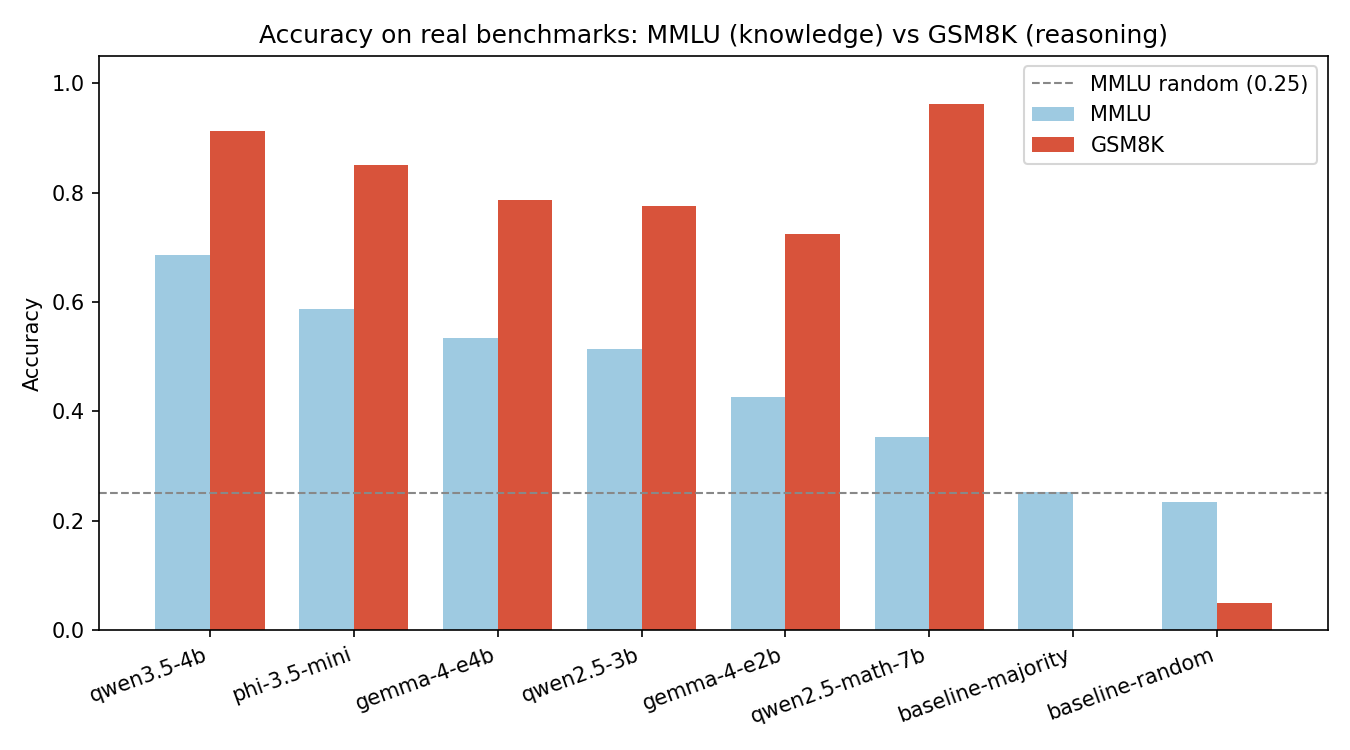
\includegraphics[width=0.8\linewidth]{images/saturation.png}
  \caption{Accuracy MMLU vs GSM8K theo model. GSM8K bám sát trần trên; MMLU trải
  rộng --- một benchmark còn ``đo được'', một benchmark đã ``bão hoà''.}
  \label{fig:saturation}
\end{figure}

\subsection{Rank-instability: chính benchmark chọn người thắng}

Đây là kết quả trung tâm. Bảng~\ref{tab:ranking} xếp hạng các model trên MMLU và
GSM8K \emph{riêng}. Trong panel năm model đa năng, thứ hạng trùng khít; nhưng
\textbf{math-specialist} làm thứ hạng \emph{rã}: nó đứng \textbf{hạng 1 GSM8K
(0.963)} nhưng \textbf{hạng 6 --- bét bảng --- trên MMLU (0.353)}, với
\texttt{rank\_shift} = 5.

\begin{table}[t]
\centering
\caption{Thứ hạng trên hai benchmark. Math-specialist lật từ hạng 6 (MMLU) lên
hạng 1 (GSM8K). Tương quan hạng Spearman $\rho = 0.14$ trên cả sáu model, và
$\rho = 0.0$ riêng nhóm $\geq 3$B.}
\label{tab:ranking}
\small
\begin{tabular}{lcccc}
\hline
\textbf{System} & \textbf{params\_b} & \textbf{rank\_mmlu} & \textbf{rank\_gsm8k} & \textbf{shift} \\
\hline
qwen3.5-4b      & 4.0 & 1 & 2 & 1 \\
phi-3.5-mini    & 3.8 & 2 & 3 & 1 \\
gemma-4-e4b     & 4.5 & 3 & 4 & 1 \\
qwen2.5-3b      & 3.1 & 4 & 5 & 1 \\
gemma-4-e2b     & 2.3 & 5 & 6 & 1 \\
qwen2.5-math-7b & 7.0 & \textbf{6} & \textbf{1} & \textbf{5} \\
\hline
\end{tabular}
\end{table}

Hệ quả định lượng: hệ số tương quan hạng \textbf{Spearman $\rho = 0.14$} cho cả sáu
model, và \textbf{$\rho = 0.0$} (không tương quan) cho riêng nhóm $\geq 3$B. Đáng
chú ý nhất: model \emph{to nhất panel} (7B) lại \emph{thua mọi model 2--4B trên
MMLU} trong khi \emph{thắng tất cả trên GSM8K}. Cần nói rõ phạm vi của kết luận này:
panel năm model đa năng \emph{vẫn} xếp hạng nhất quán giữa hai benchmark (chỉ shift
1 bậc, $\rho = 1.0$ nếu xét riêng); toàn bộ $\rho = 0.14$ là do \emph{một} model lệch
chủ đích (math-7b) gây ra. Vì vậy luận điểm không phải ``benchmark luôn đảo lộn mọi
thứ hạng'', mà là \textbf{một construct duy nhất đủ lệch so với panel là đủ để biến
``ai thắng'' thành \emph{hàm của việc chọn benchmark}} --- và đó chính là rủi ro mà
một bảng xếp hạng đơn-benchmark không bộc lộ. Hình~\ref{fig:agreement}
trực quan hoá: math-specialist nằm hẳn ngoài đám đông, ở góc dưới-phải (GSM8K cao,
MMLU thấp), phá vỡ đường chéo đồng thuận.

\begin{figure}[t]
  \centering
  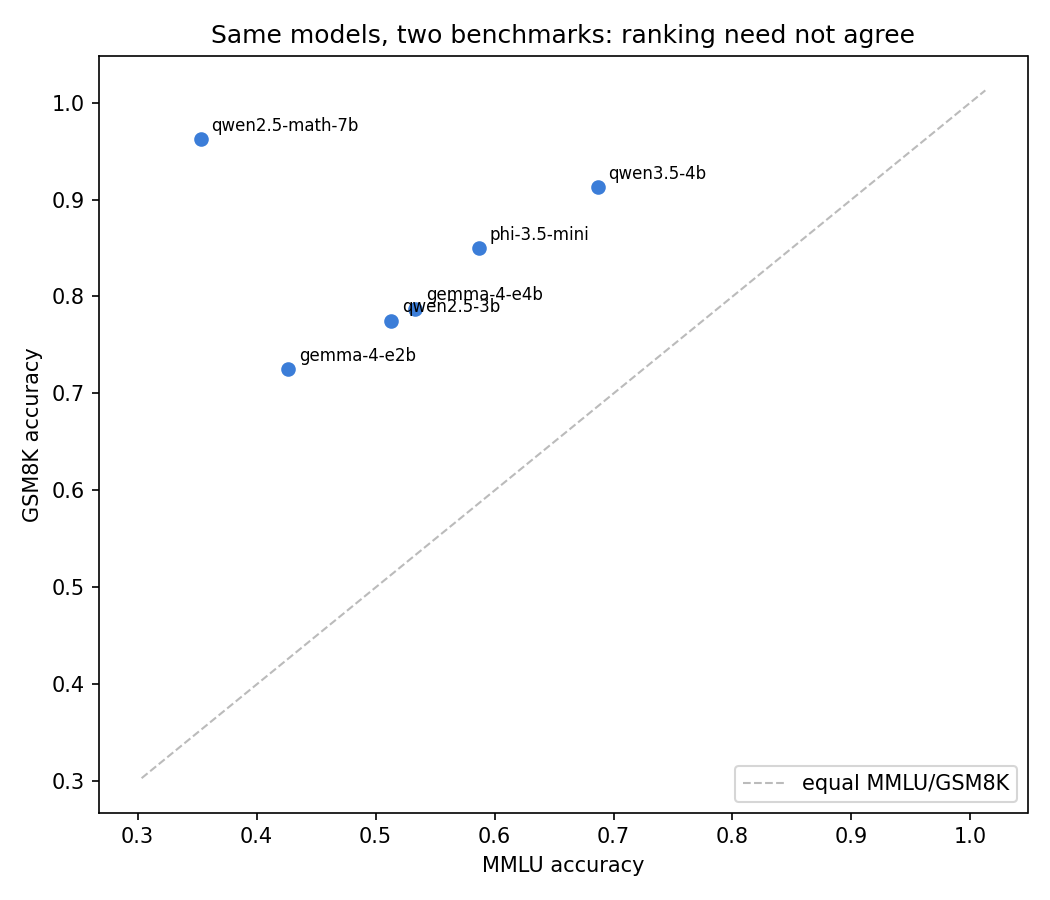
\includegraphics[width=0.7\linewidth]{images/model_agreement.png}
  \caption{Scatter MMLU $\times$ GSM8K. Năm model đa năng bám một đường đơn điệu;
  math-specialist (góc dưới-phải) phá thế đồng thuận $\Rightarrow$ thứ hạng phụ
  thuộc benchmark.}
  \label{fig:agreement}
\end{figure}

\paragraph{Minh bạch thiết kế.} Math-specialist là một \emph{đầu dò chủ đích lệch},
không thuộc panel $\sim$4B. Bản thân panel năm model đa năng xếp hạng \emph{trùng}
($\rho = 1.0$); chính việc \emph{thêm} một model lệch chuyên môn mới làm $\rho$ rã.
Nhóm khai báo rõ điều này: rank-instability là thứ phải \emph{đo}, và ở đây ta
\emph{dựng điều kiện để đo nó}, chứ không trình bày như hiện tượng tự nhiên xảy ra
ở mọi panel.

\subsection{Metric giòn: cùng câu trả lời, đổi cách chấm là sập điểm}

Bảng~\ref{tab:metricgap} cho thấy độ giòn của lớp chấm GSM8K. Với \emph{cùng một
đầu ra} của mô hình, bộ chấm \emph{naive} (lấy số đầu) cho accuracy $\approx 0$
trong khi bộ \emph{robust} (lấy số cuối) cho 0.73--0.96. Cột
\texttt{n\_robust\_only} --- số câu đúng bị bộ giòn đánh trượt --- lên tới
\textbf{58--77 trên 80 câu}.

\begin{table}[t]
\centering
\caption{GSM8K: hai bộ chấm khác nhau \emph{đúng một quyết định} (vị trí lấy số).
Chênh lệch khổng lồ $\Rightarrow$ \emph{metric $\neq$ construct}.}
\label{tab:metricgap}
\small
\begin{tabular}{lccc}
\hline
\textbf{System} & \textbf{acc\_naive} & \textbf{acc\_robust} & \textbf{n\_robust\_only} \\
\hline
qwen2.5-math-7b & 0.000 & 0.963 & 77 \\
qwen3.5-4b      & 0.013 & 0.913 & 72 \\
phi-3.5-mini    & 0.013 & 0.850 & 67 \\
gemma-4-e4b     & 0.000 & 0.788 & 63 \\
qwen2.5-3b      & 0.013 & 0.775 & 62 \\
gemma-4-e2b     & 0.000 & 0.725 & 58 \\
\hline
\end{tabular}
\end{table}

Đây là bằng chứng định lượng đậm nét cho luận điểm \emph{metric $\neq$ construct}:
năng lực thật của mô hình không đổi, nhưng một lựa chọn cài đặt tầm thường trong
lớp chấm có thể biến điểm từ 0.96 thành 0.00. Hình~\ref{fig:metricgap} minh hoạ
khoảng cách này; ví dụ cụ thể được phân tích ở Phần~\ref{sec:error}.

\begin{figure}[t]
  \centering
  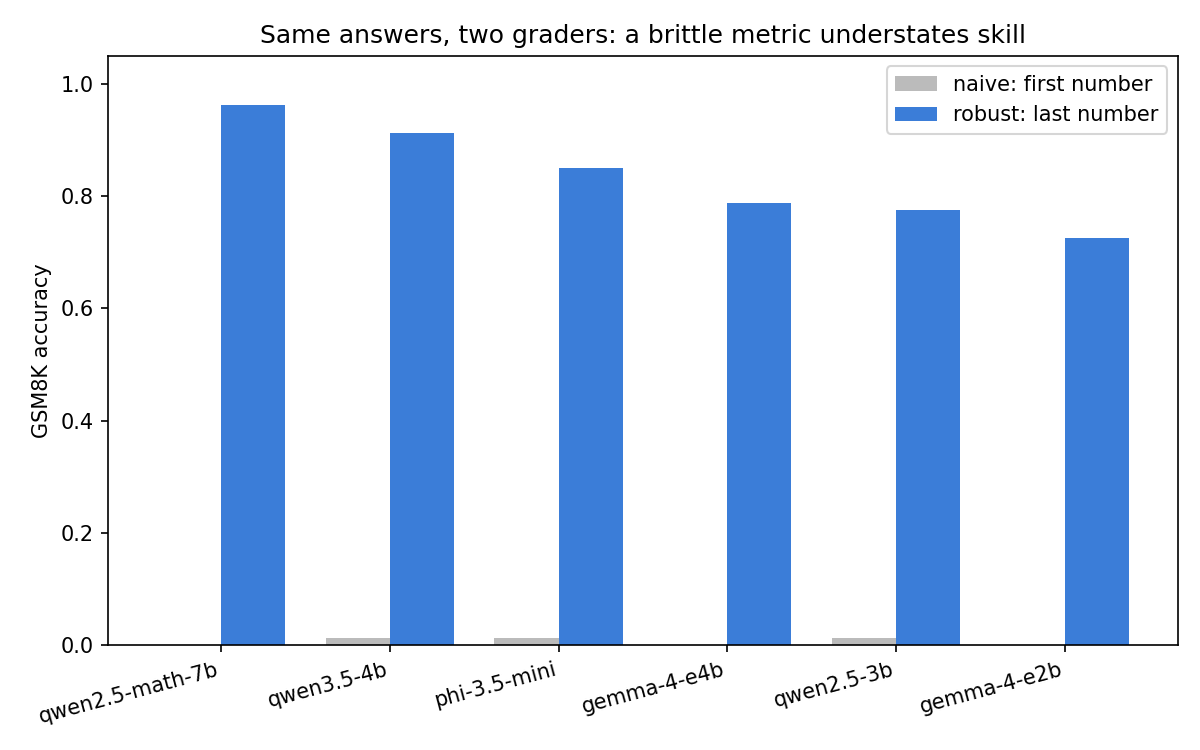
\includegraphics[width=0.8\linewidth]{images/metric_gap.png}
  \caption{GSM8K: accuracy theo bộ chấm \emph{naive} (số đầu) vs \emph{robust}
  (số cuối). Chỉ khác vị trí lấy số.}
  \label{fig:metricgap}
\end{figure}

\subsection{Phương sai construct: ``MMLU accuracy'' che giấu gì}

Hình~\ref{fig:subjects} (và \texttt{mmlu\_by\_subject.csv}) tách accuracy theo từng
môn MMLU. Cùng một model nhảy từ 0.0 ở vài môn (abstract\_algebra,
college\_mathematics) lên 1.0 ở môn khác (college\_computer\_science,
professional\_medicine). Một con số ``MMLU accuracy'' duy nhất do đó \emph{che
giấu} chênh lệch lớn giữa các môn $\Rightarrow$ ``MMLU'' không phải một construct
\emph{đồng nhất}. (Lưu ý: chỉ 2--5 câu/môn nên đây là minh hoạ định tính, không
phải ước lượng chắc theo từng môn.)

\begin{figure}[t]
  \centering
  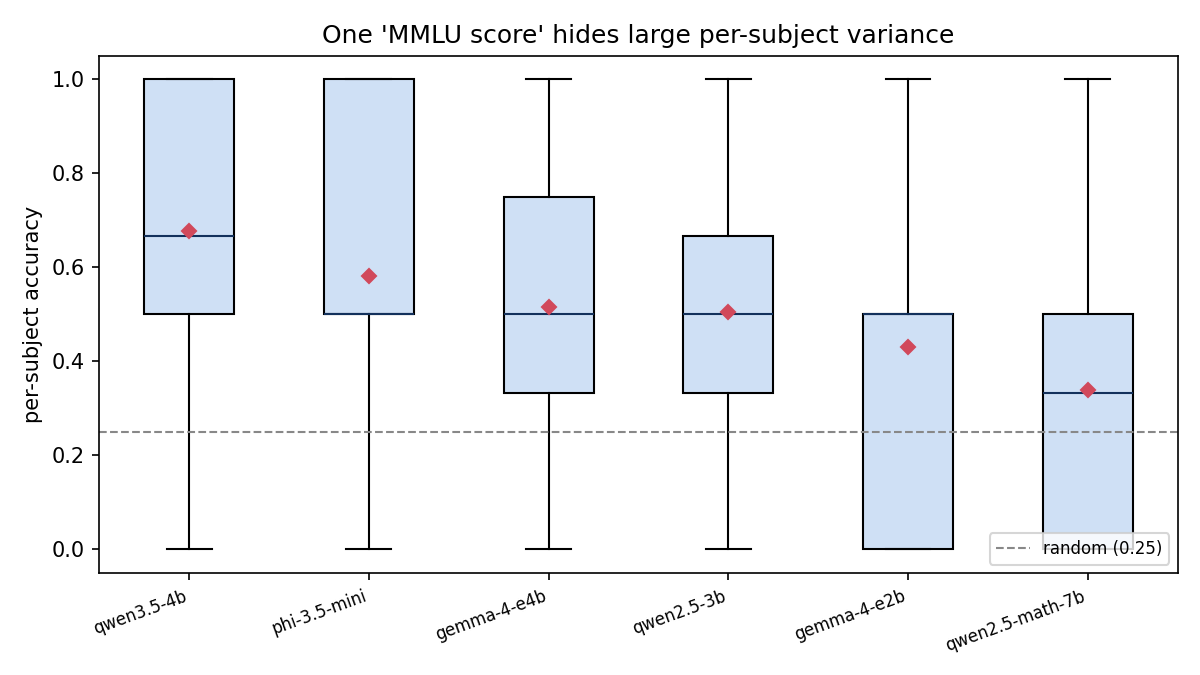
\includegraphics[width=0.85\linewidth]{images/mmlu_by_subject.png}
  \caption{Phân bố accuracy MMLU \emph{theo môn}, mỗi box ứng một model (kim cương
  đỏ = accuracy trung bình). Whisker trải gần như toàn dải $0$--$1$ cho thấy một
  con số ``MMLU accuracy'' duy nhất che giấu phương sai lớn giữa các môn $\Rightarrow$
  ``MMLU'' gộp nhiều construct khác nhau dưới một cái tên.}
  \label{fig:subjects}
\end{figure}

\subsection{Coverage: nhiễu đo lường lệch theo model}

\texttt{coverage.csv} ghi tỉ lệ câu \emph{trích được đáp án}. Trên GSM8K, coverage
= 1.0 cho mọi model; trên MMLU, coverage dao động \textbf{0.945--0.99} --- tức một
số model thi thoảng bị phạt vì \emph{không trích được đáp án} (lỗi format) chứ
không phải vì sai kiến thức. Đây là một nguồn nhiễu đo lường \emph{lệch theo model}
mà một bảng ``accuracy'' đơn thuần không bộc lộ.

\subsection{Robustness: điểm gốc dựa một phần vào format}

Bảng~\ref{tab:robust} (và Hình~\ref{fig:robust}) so accuracy gốc với accuracy trên
bản nhiễu giữ nhãn. Mọi model đều tụt \textbf{0.06--0.18}. Đáng chú ý, model
\emph{yếu MMLU nhất} (math-7b) tụt \emph{nhiều nhất} ($-0.18$): phần điểm MMLU của
nó dựa vào vị trí/format đáp án hơn là kiến thức thật --- đúng kiểu lỗ hổng mà
perturbation theo tinh thần SuperGLUE được thiết kế để phát hiện.

\begin{table}[t]
\centering
\caption{MMLU robustness: độ tụt accuracy khi đảo option / chèn distractor (giữ
nhãn). Tụt $> 0$ $\Rightarrow$ điểm gốc một phần dựa vào bề mặt câu hỏi.
\textbf{Lưu ý:} \texttt{acc\_original} ở đây tính trên \emph{đúng 50 câu được chọn
để perturbation}, nên khác accuracy toàn tập MMLU 150 câu ở Bảng~\ref{tab:accuracy}
(ví dụ math-7b: 0.46 trên tập con vs 0.353 toàn tập).}
\label{tab:robust}
\small
\begin{tabular}{lccc}
\hline
\textbf{System} & \textbf{acc\_original} & \textbf{acc\_perturbed} & \textbf{drop} \\
\hline
qwen2.5-math-7b & 0.46 & 0.28 & 0.18 \\
qwen3.5-4b      & 0.66 & 0.50 & 0.16 \\
qwen2.5-3b      & 0.56 & 0.46 & 0.10 \\
gemma-4-e4b     & 0.52 & 0.42 & 0.10 \\
phi-3.5-mini    & 0.58 & 0.50 & 0.08 \\
gemma-4-e2b     & 0.44 & 0.38 & 0.06 \\
\hline
\end{tabular}
\end{table}

\begin{figure}[t]
  \centering
  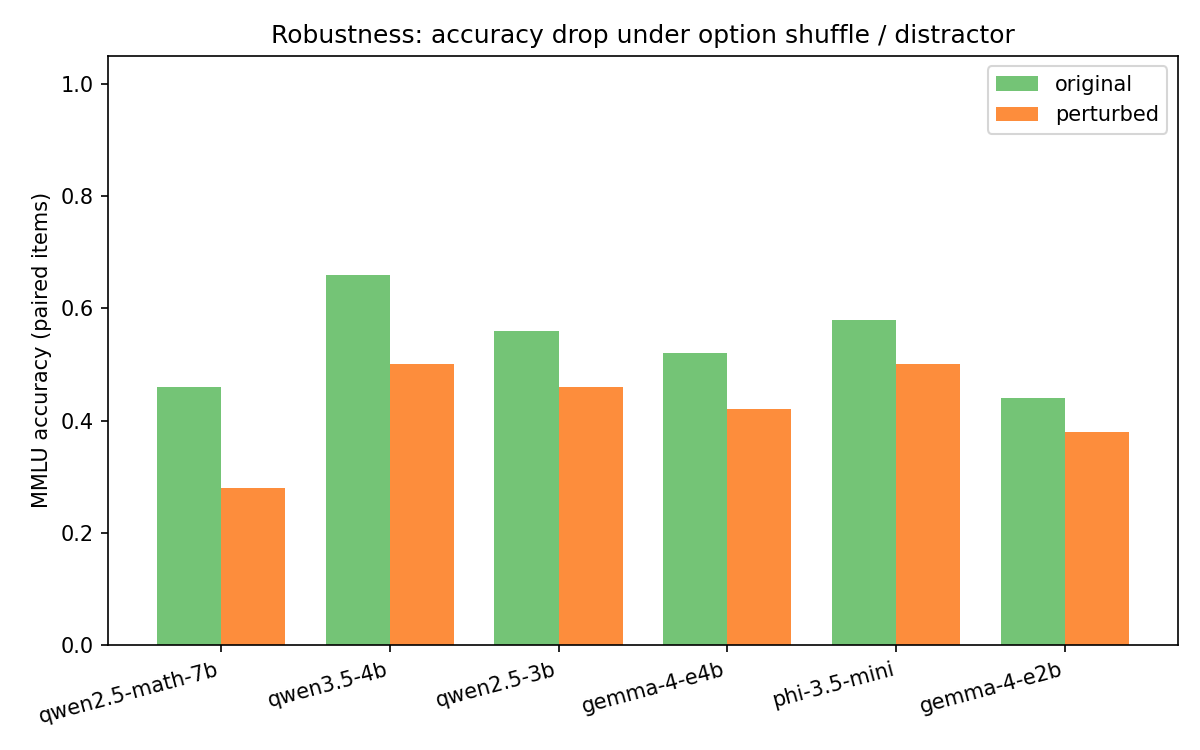
\includegraphics[width=0.8\linewidth]{images/robustness.png}
  \caption{MMLU: accuracy gốc vs accuracy sau nhiễu giữ nhãn. Mọi model đều tụt.}
  \label{fig:robust}
\end{figure}

\subsection{Cảnh báo nhiễm dữ liệu}

Một quan sát phải nêu thẳng: cả MMLU (2021) và GSM8K (2021) gần như chắc nằm trong
dữ liệu huấn luyện của các model này. Việc \textbf{GSM8K đạt $\sim$0.9 cho model
chỉ 3--4B} nhiều khả năng phản ánh \emph{trí nhớ/nhiễm dữ liệu} hơn là \emph{suy
luận} thuần. Vì vậy các điểm tuyệt đối \emph{không} nên đọc như ``năng lực thật'';
demo dùng chúng để \emph{phơi bày chính vấn đề này}, không để xếp hạng. (Robustness
tụt vừa phải cho thấy mô hình không bám chuỗi test verbatim, nhưng không loại trừ
nhiễm ở mức ngữ nghĩa.)
